\documentclass[11pt,a4paper,oneside,reqno]{amsart}

\pdfoutput=1

% \usepackage{todonotes}

\usepackage{amsmath,amssymb,amsfonts,amsthm}
\usepackage{mathtools}
% \usepackage{mathalfa}
\usepackage[T1]{fontenc}
% \usepackage{enumitem}
\usepackage{hyperref}
\usepackage[capitalise]{cleveref}
% \usepackage{upgreek}
% \usepackage{bbm}

\usepackage{tikz}
\usetikzlibrary{positioning,arrows}

\newtheorem{theorem}{Theorem}
\newtheorem{lemma}[theorem]{Lemma}
\newtheorem{corollary}[theorem]{Corollary}
\theoremstyle{definition}
\newtheorem{definition}[theorem]{Definition}
\newtheorem{example}[theorem]{Example}
\theoremstyle{remark}
\newtheorem{remark}[theorem]{Remark}
\newtheorem{conjecture}[theorem]{Conjecture}
\newtheorem{issue}[theorem]{Issue/TODO}


\newcommand{\Nat}{\mathbb{N}}
\newcommand{\Z}{\mathbb Z}
\newcommand{\Prop}{\mathsf{Prop}}
\newcommand{\UU}{\mathcal{U}}
\newcommand{\sph}[1]{{\mathbb S}^{#1}}


\newcommand{\defeq}{\vcentcolon\equiv}  
\newcommand{\refl}{\mathsf{refl}}
\newcommand{\ct}{%
  \mathchoice{\mathbin{\raisebox{0.5ex}{$\displaystyle\centerdot$}}}%
             {\mathbin{\raisebox{0.5ex}{$\centerdot$}}}%
             {\mathbin{\raisebox{0.25ex}{$\scriptstyle\,\centerdot\,$}}}%
             {\mathbin{\raisebox{0.1ex}{$\scriptscriptstyle\,\centerdot\,$}}}
}

\newcommand{\istype}[1]{\mathsf{is}\mbox{-}{#1}\mbox{-}\mathsf{type}}
\newcommand{\trunc}[2]{\mathopen{}\left\Vert #2\right\Vert_{#1}\mathclose{}}
\newcommand{\brck}[1]{\trunc{}{#1}}

\newcommand{\tproj}[3][]{\mathopen{}\left|#3\right|_{#2}^{#1}\mathclose{}}
\newcommand{\bproj}[1]{\tproj{}{#1}}

\newcommand{\isequiv}{\mathsf{isequiv}}

\newcommand{\North}{\mathsf N}
\newcommand{\South}{\mathsf S}
\newcommand{\merid}{\mathsf{merid}}
\newcommand{\pointedm}{\rightarrow_\bullet}
\newcommand{\lo}{\mathsf{loop}}

\newcommand{\idf}{\mathsf{id}}


\begin{document}

\section{Based Symmetries on the Circle}

\begin{definition}[Suspension]
 Given a type $A$, we write $\Sigma A$ for the \emph{suspension} of $A$, defined to be the (h-) pushout of $1 \leftarrow A \rightarrow 1$.
 It can be implemented as the higher inductive type with points $\North, \South$ and a family $\merid : A \to (\North = \South)$.
\end{definition}

When we later regard $\Sigma A$ as a pointed type, we implicitly choose its base point to be $\North$.


\begin{definition}[Spheres $\sph n$]
 $\sph {-1}$ is defined to be the empty type, and $\sph {n+1}$ is $\Sigma \sph n$.
\end{definition}

Given pointed types $A$ and $B$ (with implicit base points $a_0$ and $b_0$), we write $A \pointedm B$ for the type of \emph{pointed maps}: $\Sigma (f : A \to B). f(a_0) = b_0$.

\begin{lemma}[{Spheres and loops \cite[iterate Lemma 6.5.4]{HoTT}}] \label{lem:sph-loops}
 Given $n \geq 0$ and a pointed type $A$, we have
 \begin{equation}
  (\sph n \pointedm A) \simeq \Omega^n(A).
 \end{equation}
 \qed
\end{lemma}
% \begin{proof}
%  (Todo: I am sure this is a lemma in the HoTT book, but I need to find the number.)
% \end{proof}

\begin{lemma}
 The map $\gamma : \Z \to (\sph 1 \pointedm \sph 1)$, given by $\gamma_n (\lo) \defeq \lo^n$, is an equivalence of types.
\end{lemma}
\begin{proof}
 By \cref{lem:sph-loops}, this is a reformulation of the usual property that the loop space of the circle is $\Z$ \cite[Chp 8.1]{HoTT}.
\end{proof}

We denote the standard multiplication on integers by $(\_ \cdot \_)$.
Note that $\Z$ with multiplication is a monoid\footnote{Note that the definition of a monoid used here requires the carrier to be a set (a $0$-truncated type).}, and so is $(\sph 1 \pointedm \sph 1)$ with function composition.

\begin{theorem}[$\Z \simeq (\sph 1 \pointedm \sph 1)$]
 The function $\gamma$ is a monoid isomorphism between $(\Z, \_ \cdot \_)$ and $(\sph 1 \pointedm \sph 1, \_ \circ \_)$.
\end{theorem}
\begin{proof}
(Todo: I expect that this has already been recorded in the HoTT book?
If not, the following needs to be checked in detail.)

The only non-immediate property that needs to be checked is that multiplication of integers corresponds to composition of functions, in the sense that 
the following square commutes (up to homotopy):
\begin{equation}
\begin{tikzpicture}[x=7cm,y=-3cm,baseline=(current bounding box.center)]
 \tikzset{arrow/.style={shorten >=0.1cm,shorten <=.1cm,-latex}}
 \node (A) at (0,0) {$\Z \times \Z$}; 
 \node (B) at (0,1) {$(\sph 1 \pointedm \sph 1) \times (\sph 1 \pointedm \sph 1)$}; 
 \node (C) at (1,1) {$(\sph 1 \pointedm \sph 1)$}; 
 \node (D) at (1,0) {$\Z$}; 

 \draw[arrow] (A) to node [left] {$\gamma \times \gamma$} (B);
 \draw[arrow] (B) to node [above] {$(\_ \circ \_)$} (C);
 \draw[arrow] (D) to node [right] {$\gamma$} (C);
 \draw[arrow] (A) to node [above] {$(\_ \cdot \_)$} (D);
\end{tikzpicture}
\end{equation}
\end{proof}

Since the monoid of integers has exactly two invertible elements, we get the following
(note that we write $A \xrightarrow{\sim} B$ synonymously with $A \simeq B$):

\begin{corollary} \label{cor:sph1-bool}
 The type $(\sph 1 \xrightarrow{\sim}_\bullet \sph 1)$ of pointed equivalences
%  , or equivalently the type $(\sph 1 =_\bullet \sph 1)$ of pointed equalities, 
 is isomorphic to $\mathsf{Bool}$.
\end{corollary}

\section{Based Symmetries of Higher Spheres}

The suspension is a ``functor'' in the somewhat naive sense of directly writing down the usual functor laws of ordinary category theory.
We first record this observation in \cref{lem:Susp-is-functor}
before clarifying why we call the concept a \emph{wild $1$-functor} in \cref{rem:wildness}.

\begin{lemma}[Funcotrial structure of the suspension] \label{lem:Susp-is-functor}
 The suspension can canonically be given the structure of a \emph{wild $1$-functor} in the following sense:
 \begin{enumerate}
  \item \emph{Objects:} for any type $A$, we get a type $\Sigma A$.
  \item \emph{Morphisms:} given a function $f : A \to B$, we get $\Sigma f : \Sigma A \to \Sigma B$.
  \item Given functions $A \xrightarrow f B \xrightarrow g C$, we have $\Sigma(g \circ f) = \Sigma g \circ \Sigma f$. \label{eq:susp-law1}
  \item For the identity function $\idf$, we have $\Sigma \idf_A = \idf_{\Sigma A}$. \label{eq:susp-law2}
 \end{enumerate}
 \qed
\end{lemma}

\begin{remark} \label{rem:wildness}
One should in general not expect that the direct translation of categorical concepts into type theory yields well-behaved concepts.
The reason is that equalities such as the functor laws used above can only be stated using the internal equality type.
As it is well-studied, equalities play the rule of $1$-morphism in the $\infty$-category (groupoid) given by the type.
Consequently, the functor laws as formulated in the lemma above are \emph{not} mere properties but carry structure, and require coherence in order to be well-behaved.
Morally, the suspension should be regarded as an $\infty$-endofunctor on the $\infty$-category $\UU$ of types and functions.\footnote{This can be made precise, cf.\ \cite{ann-cap-kra:two-level}.}
We cannot but fortunately do not need to spell out what this means in our setting.
What happens here (and in many situations in homotopy type theory) is that certain constructions only require a \emph{finite} amount of data of the $\infty$-category.
Recall (cf.\ \cite{capKra_semisegal}) that a \emph{wild $n$-category} is a structure which carries the operations of an $n$-category without being truncated, the intuition being that it ``morally'' is an $\infty$-category with all data from level $(n+1)$ onwards omitted.
We have obvious corresponding notions of wild functors, wild natural transformations, and so on.
In our case, $n \equiv 1$ will turn out to be sufficient.
In other words, the data for a \emph{wild $1$-functor} considered in \cref{lem:Susp-is-functor} is not well-behaved, but it is ``good enough'' for everything that we do in this note.
\end{remark}



While $(\sph 1 \pointedm \sph 1)$ is a monoid, the same is not the case in general for $(\sph n \pointedm \sph n)$.
The reason is that this type is in general not a set.
However,
$\trunc 0 {\sph n \pointedm \sph n}$ is a monoid in the canonical way.

\begin{corollary} \label{cor:mon-mor}
 The morphism map $\trunc 0 {\Sigma \_} : \trunc 0 {\sph n \pointedm \sph n} \to \trunc 0 {\sph {n+1} \pointedm \sph {n+1}}$ is a monoid morphism for all $n \geq 0$.
\end{corollary}
\begin{proof}
 The monoid structure is respected by \eqref{eq:susp-law1} and \eqref{eq:susp-law2}.
%  (Todo: This needs to be worked out.
%  The statement that it is an equivalence of types should hopefully follow from the Freudenthal suspension theorem \cite[Thm 8.6.4]{HoTT}. However, we need to be careful: The map $\sigma$ in that theorem is not the same as the map $\Sigma \_$ we have here.
%  This is why the potentially useful formulations in \cite[Cor 8.6.14]{HoTT} and \cite[Thm 8.6.17]{HoTT} do not solve this immediately.
%  As Pierre has pointed out, the case for $n + 1 = 2$ needs a proof as well, since Freudenthal only works for $n \geq 2$.
%  
%  The statement that the monoid structure is respected follows from \eqref{eq:susp-law1} and \eqref{eq:susp-law2}.)
\end{proof}

\section{Based Symmetries on Higher Spheres}

The goal of this section is to improve the result of 
\cref{cor:mon-mor} to the following:

\begin{theorem} \label{thm:mon-iso}
The monoid morphism
\begin{equation}
 \trunc 0 {\Sigma \_} : \trunc 0 {\sph n \pointedm \sph n} \to \trunc 0 {\sph {n+1} \pointedm \sph {n+1}}
\end{equation}
is an isomorphism of monoids for all $n \geq 1$. 
\end{theorem}

Our strategy for proving \cref{thm:mon-iso} is to apply the
Freudenthal suspension theorem \cite[Thm 8.6.4]{HoTT}. 
Since we have $(\sph n \pointedm \sph n) \simeq \Omega^n(\sph n)$ and thus $\trunc 0 {\sph n \pointedm \sph n} = \pi_n(\sph n)$, it might seem as if 
the desired statement is already given by \cite[Cor 8.6.15]{HoTT}.
Unfortunately, we need to be careful: 
The Freudenthal suspension theorem makes a statement about the map
\begin{equation}
 \sigma : X \to \Omega(\Sigma X) : x \mapsto \mathsf{merid}(x) \ct \mathsf{merid}(x_0)^{-1},
\end{equation}
the unit of the adjunction $\Sigma \dashv \Omega$.
The isomorphism in \cite[Cor 8.6.15]{HoTT}
is given by $\mathsf{ap}^n_\sigma$.
A priori, this function has an unknown relationship with the map $\Sigma \_$ that we consider in \cref{thm:mon-iso}.
The key to proving \cref{thm:mon-iso} is thus showing that these maps are the same up to canonical isomorphism, i.e.\ commutation of the following square:

\begin{equation} \label{eq:needs-to-commute}
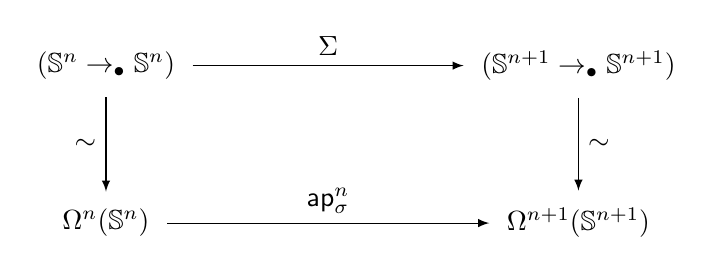
\begin{tikzpicture}[x=6cm,y=-2cm,baseline=(current bounding box.center)]
 \tikzset{arrow/.style={shorten >=0.1cm,shorten <=.1cm,-latex}}
 \node (A) at (0,0) {$(\sph n \pointedm \sph n)$}; 
 \node (B) at (0,1) {$\Omega^n(\sph n)$}; 
 \node (C) at (1,1) {$\Omega^{n+1}(\sph {n+1})$}; 
 \node (D) at (1,0) {$(\sph {n+1} \pointedm \sph {n+1})$}; 

 \draw[arrow] (A) to node [left] {$\sim$} (B);
 \draw[arrow] (B) to node [above] {$\mathsf{ap}^n_\sigma$} (C);
 \draw[arrow] (D) to node [right] {$\sim$} (C);
 \draw[arrow] (A) to node [above] {$\Sigma$} (D);
\end{tikzpicture}
\end{equation}

Our argument for this is the concatenation of the following lemmas.

\begin{lemma} \label{lem:ap-Sigma}
 Let $X$ be a pointed type and $f \equiv (f_0, f_1) : A \pointedm B$ be a pointed function.
 The following square commutes:
\begin{equation}
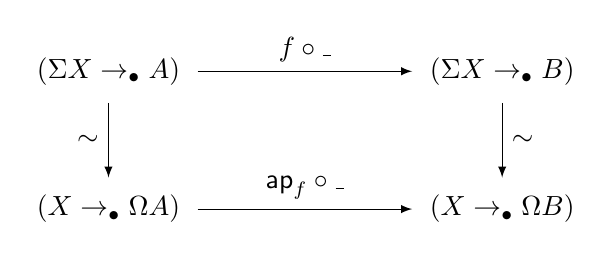
\begin{tikzpicture}[x=5cm,y=-1.75cm,baseline=(current bounding box.center)]
 \tikzset{arrow/.style={shorten >=0.1cm,shorten <=.1cm,-latex}}
 \node (A) at (0,0) {$(\Sigma X \pointedm A)$}; 
 \node (D) at (1,0) {$(\Sigma X \pointedm B)$}; 
 \node (B) at (0,1) {$(X \pointedm \Omega A)$}; 
 \node (C) at (1,1) {$(X \pointedm \Omega B)$}; 

 \draw[arrow] (A) to node [above] {$f \circ \_$} (D);
 \draw[arrow] (A) to node [left] {$\sim$} (B);
 \draw[arrow] (B) to node [above] {$\mathsf{ap}_f \circ \_$} (C);
 \draw[arrow] (D) to node [right] {$\sim$} (C);
\end{tikzpicture}
\end{equation}
\end{lemma}
\begin{proof}
 By calculation.
%  Starting with $f_0 : \Sigma X \to A$ and $f_1 : f_0(N) = a_0$ and checking where this pair is mapped if we go first down and then right, we get:
We start in the top left corner with $g_0 : \Sigma X \to A$ and $g_1 : g_0(N) = a_0$. If we go first down, then right, we get the following, where we omit the proofs that the functions are pointed:
\begin{equation}
 \begin{alignedat}{5}
  &\quad && g_0 : \Sigma X \to A & \\
  \mapsto &&& \lambda x. g_1^{-1} \ct \mathsf{ap}_{g_0}(\mathsf{merid}(x) \ct \mathsf{merid}(x_0)^{-1}) \ct g_1 : X \to \Omega A \\
  \mapsto &&& \lambda x. f_1^{-1} \ct \mathsf{ap}_{f_0}(g_1)^{-1} \ct  \mathsf{ap}_{f_0 \circ g_0}(\mathsf{merid}(x) \ct \mathsf{merid}(x_0)^{-1}) \ct \mathsf{ap}_{f_0}(g_1) \ct f_1 : X \to \Omega B
 \end{alignedat}
\end{equation}
If we go first right, then down, we get:
\begin{equation}
 \begin{alignedat}{5}
  &\quad && g_0 : \Sigma X \to A & \\
  \mapsto &&&  f_0 \circ g_0 : \Sigma X \to B \\
  \mapsto &&& \lambda x. f_1^{-1} \ct \mathsf{ap}_{f_0}(g_1)^{-1} \ct  \mathsf{ap}_{f_0 \circ g_0}(\mathsf{merid}(x) \ct \mathsf{merid}(x_0)^{-1}) \ct \mathsf{ap}_{f_0}(g_1) \ct f_1 : X \to \Omega B
 \end{alignedat}
\end{equation}
The proofs that the functions are pointed are the canonical ones and coincide as well. (todo: if we have a formalisation, we can refer to that.)
\end{proof}

\begin{lemma}\label{lem:iterated-ap-Sigma}
 For all $n \geq 0$ and $f$ as above, the diagram
\begin{equation}
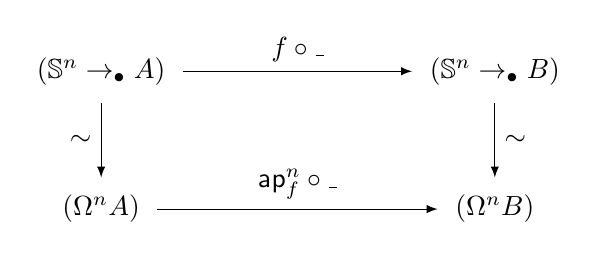
\begin{tikzpicture}[x=5cm,y=-1.75cm,baseline=(current bounding box.center)]
 \tikzset{arrow/.style={shorten >=0.1cm,shorten <=.1cm,-latex}}
 \node (A) at (0,0) {$(\sph n \pointedm A)$}; 
 \node (D) at (1,0) {$(\sph n \pointedm B)$}; 
 \node (B) at (0,1) {$(\Omega^n A)$}; 
 \node (C) at (1,1) {$(\Omega^n B)$}; 

 \draw[arrow] (A) to node [above] {$f \circ \_$} (D);
 \draw[arrow] (A) to node [left] {$\sim$} (B);
 \draw[arrow] (B) to node [above] {$\mathsf{ap}_f^n \circ \_$} (C);
 \draw[arrow] (D) to node [right] {$\sim$} (C);
\end{tikzpicture}
\end{equation}
 commutes.
\end{lemma}
\begin{proof}
 By induction on $n$. The case $n \equiv 0$ is trivial.
 The step from $n$ to $n+1$ is an application of \cref{lem:ap-Sigma}.
\end{proof}

The next lemma is a standard property of adjunctions, here worked out explicitly for $\Sigma \dashv \Omega$:
\begin{lemma} \label{lem:adj-prop}
 For pointed types $C$ and $D$, the following commutes:
\begin{equation}
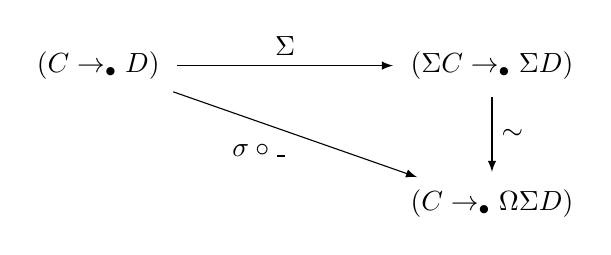
\begin{tikzpicture}[x=5cm,y=-1.75cm,baseline=(current bounding box.center)]
 \tikzset{arrow/.style={shorten >=0.1cm,shorten <=.1cm,-latex}}
 \node (A) at (0,0) {$(C \pointedm D)$}; 
 \node (D) at (1,0) {$(\Sigma C \pointedm \Sigma D)$}; 
 \node (C) at (1,1) {$(C \pointedm \Omega \Sigma D)$}; 

 \draw[arrow] (A) to node [above] {$\Sigma$} (D);
 \draw[arrow] (A) to node [below left] {$\sigma \circ \_$} (C);
 \draw[arrow] (D) to node [right] {$\sim$} (C);
\end{tikzpicture}
\end{equation}
\end{lemma}
\begin{proof}
 By easy calculation.
\end{proof}

\begin{lemma} \label{lem:what-commutes-commutes}
 The diagram \eqref{eq:needs-to-commute} commutes.
\end{lemma}
\begin{proof}
 Consider the following:
\begin{equation}
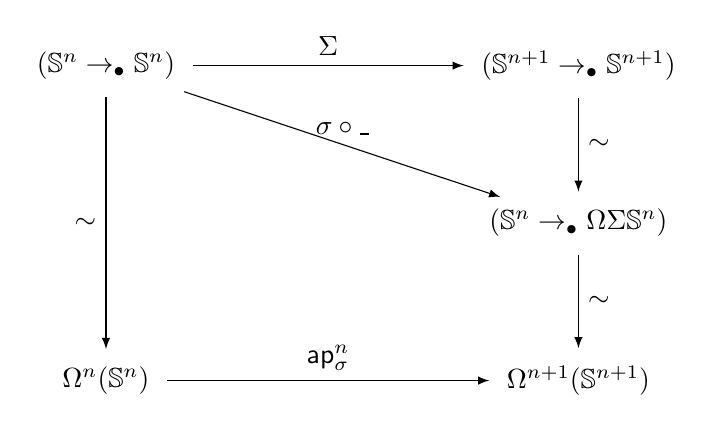
\begin{tikzpicture}[x=6cm,y=-2cm,baseline=(current bounding box.center)]
 \tikzset{arrow/.style={shorten >=0.1cm,shorten <=.1cm,-latex}}
 \node (A) at (0,0) {$(\sph n \pointedm \sph n)$}; 
 \node (B) at (0,2) {$\Omega^n(\sph n)$}; 
 \node (C) at (1,2) {$\Omega^{n+1}(\sph {n+1})$}; 
 \node (D) at (1,0) {$(\sph {n+1} \pointedm \sph {n+1})$}; 
 \node (E) at (1,1) {$(\sph n \pointedm \Omega \Sigma \sph n)$};
 
 \draw[arrow] (A) to node [left] {$\sim$} (B);
 \draw[arrow] (B) to node [above] {$\mathsf{ap}^n_\sigma$} (C);
%  \draw[arrow] (D) to node [right] {$\sim$} (C);
 \draw[arrow] (A) to node [above] {$\Sigma$} (D);
 \draw[arrow] (D) to node [right] {$\sim$} (E);
 \draw[arrow] (E) to node [right] {$\sim$} (C);
 \draw[arrow] (A) to node [above] {$\sigma \circ \_$} (E);
\end{tikzpicture}
\end{equation}
The top triangle commutes by \cref{lem:adj-prop}.
The bottom quadrangel commutes by \cref{lem:iterated-ap-Sigma}.
\end{proof}

We are now ready to prove
\cref{thm:mon-iso}, i.e.\ that 
\begin{equation}
 \trunc 0 {\Sigma \_} : \trunc 0 {\sph n \pointedm \sph n} \to \trunc 0 {\sph {n+1} \pointedm \sph {n+1}}
\end{equation}
is an isomorphism of monoids for all $n \geq 1$. 

\begin{proof}[Proof of \cref{thm:mon-iso} for the case $n \geq 2$]
 Consider the set-truncation of digram \eqref{eq:needs-to-commute}.
 By the Freudenthal suspension theorem, the bottom horizontal map is an equivalence for $n \geq 2$.
 Since the vertical maps are always equivalences, by \cref{lem:what-commutes-commutes}, the top vertical map $\trunc 0 \Sigma$ is an equivalence.
 By \cref{cor:mon-mor}, this map preserves the monoid structure.
\end{proof}

\begin{proof}[Proof of \cref{thm:mon-iso} for the cases $n \equiv 1$]
 TODO: Here is the connection to Pierre's and Marc's writeup!
\end{proof}

From this, we immediately get:

\begin{theorem} \label{thm:Sn-bool}
 The type
 $\trunc 0 {\sph n \xrightarrow{\sim}_\bullet \sph n}$
is equivalent to $\mathsf{Bool}$ for all $n \geq 1$.
\end{theorem}
\begin{proof}
 By (TODO: connection to Pierre and Marc's writeup!), the statement holds for $n \equiv 1$.
 By \cref{thm:mon-iso}, it holds for all $n$.
\end{proof}



\section{Unbased Symmetries}

The next (and, at the moment, final) step is from the based symmetries considered above to unbased symmetries, i.e.\ from equivalences $\sph n \xrightarrow{\sim}_\bullet \sph n$ to $\sph n \xrightarrow{\sim} \sph n$ (and thus $\sph n = \sph n$).
We start with a lemma allowing us the removal of base points:
\begin{lemma} \label{lem:rm-base-points}
 For a type $B$ and $A$ with explicitly given point $a_0$, we have
 \begin{equation}
  (A \to B) \; \simeq  \; \Sigma (b : B). (A,a_0) \to_\bullet (B,b).
 \end{equation}
\end{lemma}
\begin{proof}
 ``Singleton-contraction.''
\end{proof}


\begin{lemma} \label{lem:eqv-to-bool}
 For all $x : \sph n$ with $n \geq 1$, we have the following equivalence:
 \begin{equation}
%   \trunc 0 {(\sph n, \North) \to_\bullet (\sph n, x), \lambda \_ . x} \xrightarrow{\sim}_\bullet (\mathsf{Bool}, \mathsf{true}).
  \trunc {-1} {\trunc 0 {(\sph n, \North) \to_\bullet (\sph n, x)} \simeq \mathsf{Bool}}.
 \end{equation}
\end{lemma}
\begin{proof}
 By induction on $x$.
 Since the goal is a proposition, it is enough to check the cases for the point constructors. For $\North$, this is given by 
 \cref{thm:Sn-bool}. Note that it is always true that $(B = C)$ implies $(A \to_\bullet B) \simeq (A \to_\bullet C)$;
 thus, a single equivalence on $\sph n$ swapping $\North$ and $\South$ is suffices to cover the case $\South$.
 There is a canonical such equivalence which reverses all meridians.
\end{proof}


\begin{issue}
 I think the proof of \cref{lem:eqv-to-bool} is correct, but there would be a more elegant argument.
 If we want to inhabit a family of $(n-1)$-types over a pointed $n$-connected type, then it suffices to inhabit the family at the base point. This is directly applicable in \cref{lem:eqv-to-bool}. Moreover, if we start with $n \geq 2$, we can remove the propositional truncation, saving us the step from \cref{lem:mainlemma} to \cref{thm:symmetries-two-components}.
 Coincidentally (?), \cref{lem:grp-iso} also needs to be treated separately for $n < 2$, as Pierre has pointed out.
 We could restructure the argument so that we only do the case $n \geq 2$ here, and then maybe combine with the first approach?
\end{issue}


\begin{lemma} \label{lem:sn-bool}
 For $n \geq 1$, we have
 \begin{equation}
  \trunc {-1} {\big(\Sigma (x : \sph n). \trunc 0 {(\sph n , \North) \to_\bullet (\sph n, x)\big)} \; \simeq \; \sph n \times \mathsf{Bool}}.
 \end{equation}
\end{lemma}
\begin{proof}
 By taking the total spaces of the result of \cref{lem:eqv-to-bool}.
\end{proof}

\begin{lemma} \label{lem:rm-truncs}
 For all types $A$, families $B$, and $k \geq -2$, we have
 \begin{equation}
  \trunc k {\Sigma (a : A). B(a)} \; \simeq \; \trunc k {\Sigma (a : A). \trunc k {B(a)}}.
 \end{equation}
 \qed
\end{lemma}

Curiously, the main theorem works for $n \equiv 0$, even though the above statements fail for this case (the requirement $n \geq 1$ trickles down from \cref{lem:grp-iso}).
\begin{lemma} \label{lem:mainlemma}
 For all $n \geq 0$, the type of symmetries of $\sph n$ merely has exactly two connected components.
 In other words,
 \begin{equation}
  \trunc {-1} {\trunc 0 {\sph n = \sph n} = \mathsf{Bool}}.
 \end{equation}
\end{lemma}
\begin{proof}
 The case $n \equiv 0$ is easily checked.
 For $n \geq 1$, we have the following chain of ``mere equivalences'' (i.e.\ the chain is to be understood in the ``truncation monad'', i.e.\ every step is only ``merely true''):
  \begin{alignat}{5}
  &&&\trunc 0 {\sph n = \sph n} \\
  \textit{by }\cref{lem:rm-base-points} \qquad &\simeq &\quad& \trunc 0 {\Sigma(x : \sph n).(\sph n, \North) \xrightarrow{\sim}_\bullet (\sph n, x)}  \\
  \textit{by }\cref{lem:rm-truncs} \qquad &\simeq && \trunc 0 {\Sigma(x : \sph n).\trunc 0 {(\sph n, \North) \xrightarrow{\sim}_\bullet (\sph n, x)}}  \\
  \textit{by }\cref{lem:sn-bool} \qquad &\simeq && \trunc 0 {\sph n \times \mathsf{Bool}}  \\
  \textit{ } \qquad &\simeq && \trunc 0 {\sph n} \times \trunc 0 {\mathsf{Bool}}    \\
  \textit{spheres are connected} \qquad &\simeq && \mathsf{Bool}
 \end{alignat}
(Todo: is the formulation in parentheses above understandable?)
\end{proof}

We can get rid of the propositional truncation:
\begin{theorem} \label{thm:symmetries-two-components}
 For all $n \geq 0$, the type of symmetries of $\sph n$ has exactly two connected components.
 In other words,
 \begin{equation}
  \trunc 0 {\sph n = \sph n} = \mathsf{Bool}.
 \end{equation}
\end{theorem}
\begin{proof}
 The type 
 \begin{equation}
  \left(\trunc 0 {\sph n = \sph n}, \tproj {0} \refl\right) \xrightarrow{\sim}_\bullet (\mathsf{Bool},\mathsf{true})
 \end{equation}
 is a proposition.
 It follows from \cref{lem:mainlemma} and implies the claimed equality.
\end{proof}



% % % SOMETHING NOT RIGHT HERE; THIS IS TAKEN OUT FOR NOW
% This gives us the following result for the circle:
% 
% \begin{theorem}
% We have:
%  \begin{equation}
%   (\sph 1 = \sph 1) = (\sph 1 + \sph 1).
%  \end{equation}
% \end{theorem}
% \begin{proof}
%  This follows by combining 
%  \cref{cor:sph1-bool} with
%  \cref{lem:rm-base-points}.
% \end{proof}
% 
% For higher spheres, some more work is needed.

\appendix

\section{Other Notes}

The following could be useful (maybe).

\begin{definition}[{reduced suspension \cite[Rem 8.6.3]{HoTT}}]
 Given a pointed type $A$ with base point $a_0$, the \emph{reduced suspension} $\Sigma^w A$ is the following higher inductive type:
 \begin{align*}
  & \textit{inductive} \; \Sigma^w A \\
  & \quad \North : \Sigma^w A \\
  & \quad \merid : A \to \North = \North \\
  & \quad \mathsf{base} : \merid(a_0) = \refl
 \end{align*}
\end{definition}

\begin{lemma}[{$\Sigma^w = \Sigma$ \cite[Rem 8.6.3]{HoTT}}]
 For a pointed type $A$, the suspension is equivalent to the reduced suspension.
\end{lemma}
\begin{proof}
  $\Sigma A \to \Sigma^w A$ is given by
 \begin{align*}
  & \North \mapsto \North \\
  & \South \mapsto \North \\
  & \merid(a) \mapsto \merid(a).\\
%  \end{align*}
  \intertext{Let the base point of $A$ be $a_0$.
  $\Sigma^w A \to \Sigma A$ is given by}
%  \begin{align*}
  & \North \mapsto \North \\
  & \merid(a) \mapsto \merid(a) \ct \merid(a_0)^{-1} \\
  & \mathsf{base} \mapsto \mathsf{syminv}.
 \end{align*}
 An easy calculation shows that these are inverses.
\end{proof}



\bibliographystyle{plain}
\bibliography{bib}


\end{document}
